% Options for packages loaded elsewhere
\PassOptionsToPackage{unicode}{hyperref}
\PassOptionsToPackage{hyphens}{url}
%
\documentclass[
]{article}
\usepackage{amsmath,amssymb}
\usepackage{iftex}
\ifPDFTeX
  \usepackage[T1]{fontenc}
  \usepackage[utf8]{inputenc}
  \usepackage{textcomp} % provide euro and other symbols
\else % if luatex or xetex
  \usepackage{unicode-math} % this also loads fontspec
  \defaultfontfeatures{Scale=MatchLowercase}
  \defaultfontfeatures[\rmfamily]{Ligatures=TeX,Scale=1}
\fi
\usepackage{lmodern}
\ifPDFTeX\else
  % xetex/luatex font selection
\fi
% Use upquote if available, for straight quotes in verbatim environments
\IfFileExists{upquote.sty}{\usepackage{upquote}}{}
\IfFileExists{microtype.sty}{% use microtype if available
  \usepackage[]{microtype}
  \UseMicrotypeSet[protrusion]{basicmath} % disable protrusion for tt fonts
}{}
\makeatletter
\@ifundefined{KOMAClassName}{% if non-KOMA class
  \IfFileExists{parskip.sty}{%
    \usepackage{parskip}
  }{% else
    \setlength{\parindent}{0pt}
    \setlength{\parskip}{6pt plus 2pt minus 1pt}}
}{% if KOMA class
  \KOMAoptions{parskip=half}}
\makeatother
\usepackage{xcolor}
\usepackage[margin=1in]{geometry}
\usepackage{graphicx}
\makeatletter
\def\maxwidth{\ifdim\Gin@nat@width>\linewidth\linewidth\else\Gin@nat@width\fi}
\def\maxheight{\ifdim\Gin@nat@height>\textheight\textheight\else\Gin@nat@height\fi}
\makeatother
% Scale images if necessary, so that they will not overflow the page
% margins by default, and it is still possible to overwrite the defaults
% using explicit options in \includegraphics[width, height, ...]{}
\setkeys{Gin}{width=\maxwidth,height=\maxheight,keepaspectratio}
% Set default figure placement to htbp
\makeatletter
\def\fps@figure{htbp}
\makeatother
\setlength{\emergencystretch}{3em} % prevent overfull lines
\providecommand{\tightlist}{%
  \setlength{\itemsep}{0pt}\setlength{\parskip}{0pt}}
\setcounter{secnumdepth}{-\maxdimen} % remove section numbering
\newlength{\cslhangindent}
\setlength{\cslhangindent}{1.5em}
\newlength{\csllabelwidth}
\setlength{\csllabelwidth}{3em}
\newlength{\cslentryspacingunit} % times entry-spacing
\setlength{\cslentryspacingunit}{\parskip}
\newenvironment{CSLReferences}[2] % #1 hanging-ident, #2 entry spacing
 {% don't indent paragraphs
  \setlength{\parindent}{0pt}
  % turn on hanging indent if param 1 is 1
  \ifodd #1
  \let\oldpar\par
  \def\par{\hangindent=\cslhangindent\oldpar}
  \fi
  % set entry spacing
  \setlength{\parskip}{#2\cslentryspacingunit}
 }%
 {}
\usepackage{calc}
\newcommand{\CSLBlock}[1]{#1\hfill\break}
\newcommand{\CSLLeftMargin}[1]{\parbox[t]{\csllabelwidth}{#1}}
\newcommand{\CSLRightInline}[1]{\parbox[t]{\linewidth - \csllabelwidth}{#1}\break}
\newcommand{\CSLIndent}[1]{\hspace{\cslhangindent}#1}
\usepackage{booktabs}
\usepackage{longtable}
\usepackage{array}
\usepackage{multirow}
\usepackage{wrapfig}
\usepackage{float}
\usepackage{colortbl}
\usepackage{pdflscape}
\usepackage{tabu}
\usepackage{threeparttable}
\usepackage{threeparttablex}
\usepackage[normalem]{ulem}
\usepackage{makecell}
\usepackage{xcolor}
\ifLuaTeX
  \usepackage{selnolig}  % disable illegal ligatures
\fi
\IfFileExists{bookmark.sty}{\usepackage{bookmark}}{\usepackage{hyperref}}
\IfFileExists{xurl.sty}{\usepackage{xurl}}{} % add URL line breaks if available
\urlstyle{same}
\hypersetup{
  pdftitle={Exploring non-parametric and semi-parametric selectivity using 2d and 3d AR(1) smoothers},
  pdfauthor={Grant Adams and Cole Monnahan},
  hidelinks,
  pdfcreator={LaTeX via pandoc}}

\title{Exploring non-parametric and semi-parametric selectivity using 2d
and 3d AR(1) smoothers}
\author{Grant Adams and Cole Monnahan}
\date{2023-10-17}

\begin{document}
\maketitle

\hypertarget{executive-summary}{%
\section{Executive Summary}\label{executive-summary}}

Fishery age composition residuals have suggested misfit for this model
for several decades, and has been a point of concern for the PT and SSC.
More flexible configurations for fishery selectivity need to be
explored. Facilitation of a new suite of more flexible non-parametric
and semi-parametric selectivities in a more rigorous statistical
framework requires moving away from ADMB and toward its replacement TMB.
We thus ported model 19.1a (the 2022 final model) to TMB and demonstrate
nearly identical estimates. We call the TMB version of 19.1a model 23.0
to reflect the change in software framework. We then used model 23.0 to
explore a suite of fisheries selectivities which vary in their
flexibility and where that flexibility is permitted. We conclude that
two non-parametric models would make for an improved fisheries
selectivity formulation based on analyzing OSA residuals, AIC model
selection, and performance in projected selectivity. The models are
23.0a which uses a 2D AR(1) model, and 23.0b which uses a so-called 3D
AR(1) process that parses age, year, and cohort correlations from the
data. These models are not expected to greatly impact management advice,
but we believe their improved performance and projection capabilities
make for a better stock assessment moving forward.

\textbf{The authors recommend moving to 23.0 this year, and leave it up
to PT discretion whether to adopt 23.0a or 23.0b this year.}

\hypertarget{proposed-models}{%
\section{Proposed models}\label{proposed-models}}

\hypertarget{model-23.0-bridging-from-admb-to-template-model-builder}{%
\subsection{Model 23.0: Bridging from ADMB to Template Model
Builder}\label{model-23.0-bridging-from-admb-to-template-model-builder}}

Template Model Builder {[}TMB; Kristensen et al. (2016){]} is a software
platform designed to estimate complex, non-linear hierarchical models.
Its primary feature is the ability to efficiently apply the Laplace
approximation to the marginal likelihood, so that process errors can be
estimated using standard numerical optimization (Skaug and Fournier
2006). It is widely seen as the successor to ADMB, which has limited
Laplace approximation capabilities and thus a penalized maximum
likelihood approach is generally taken (i.e., process errors fixed and
random effects estimated as fixed effects). Despite this important
advantage, there have been relatively few implementations for stock
assessments in the North Pacific. TMB is used more widely in other
areas, such as WHAM (Stock and Miller 2021) on the US East Coast, and
SAM (Nielsen and Berg 2014) in Europe. A WHAM version of the GOA pollock
assessment was presented to the Plan Team in 2022, but there are
advantages to using a bespoke model like the ADMB version developed by
Martin Dorn and used for decades. Here we present a direct port of the
2022 accepted ADMB model 19.1a to TMB. Due to a change in software we
name this model 23.0, although our initial goal is to match model 19.1a
as close as possible.

We therefore converted the bespoke ADMB model to TMB. There are a few
important differences between ADMB and TMB in terms of syntax and
functionality relevant to stock assessments. TMB has no native phased
estimation capabilities (although there is an R function that serves a
similar purpose) so all parameters are estimated simultaneously starting
from their initial values. We used the 19.1a MLE estimates as initial
values in model 23 and were able to obtain the same model predictions,
and when optimized from there the same standard errors (uncertainties)
for parameters and derived quantities (Fig 1.). TMB does not have an
equivalent to ADMB's ``dev\_vector'' parameter class which penalizes a
vector to have a mean of zero. Model 19.1a uses this feature by
estimating a single mean in addition to the vector. When converting to a
standard unpenalized vector, a degree of freedom is lost. The means are
thus fixed at arbitrary values and mathematically the two become
equivalent.

\begin{figure}
\centering
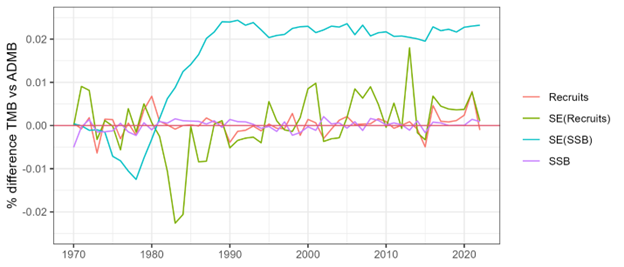
\includegraphics{Results/Figure1_time_series_of_se.png}
\caption{\textbf{Figure 1.} Results of bridging the ADMB 19.1a model to
TMB model 23.0. Shown are estimates and standard errors (SE) for two key
outputs, annual recruitment (in billions) and spawning stock biomass
(SSB; in M t). The differences, calculated as (TMB-ADMB)/ADMB are very
small, typically less than 0.02\%, and presumably due to differences in
the optimizer and precision of data inputs.}
\end{figure}

\hypertarget{non-parametric-and-semi-parametric-fisheries-selectivity}{%
\subsection{Non-parametric and semi-parametric fisheries
selectivity}\label{non-parametric-and-semi-parametric-fisheries-selectivity}}

This stock has had persistent residual patterns in the fishery age
composition data for many years, particularly for age 4 and 5 (Fig. 2).
This has been a concern of the PT for many years. For instance

\emph{The GOA Plan Team in its November 2019 minutes recommended the
author examine fishery selectivity, as persistent patterns in the
catch-at-age residuals may represent artifacts of the selectivity
functional form used.}

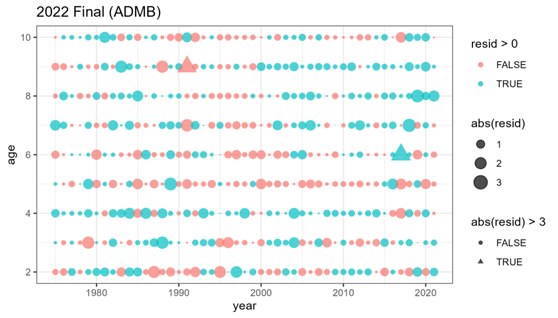
\includegraphics{Results/Figure2_admb_osa.png} In 2022 several ad hoc
approaches were explored which demonstrated that a more flexible
fisheries selectivity form could reduce the residual patterns. However,
these approaches were difficult to justify and relied on arbitrarily
setting likelihood penalties of time-varying selectivity curves. Instead
it would be ideal to explore more flexible selectivity options based on
published literature, and estimate the amount of flexibility from the
data. We therefore use model 23.0 to explore alternative selectivity
parameterizations. First, we review three important classes of
hierarchical modeling approaches that can be used for selectivity:
parametric, non-parametric, and semi-parametric functions.

\hypertarget{parametric-models}{%
\subsubsection{Parametric models}\label{parametric-models}}

Parametric selectivity curves are mathematical functions that have
typically 2-4 parameters that define a specific form or shape (often
asymptotic or dome shaped). Some common functions selected for
parametric selectivity are: double normal, logistic, and double
logistic. The pollock model has used double logistic historically. They
are usually selected based on hypothesized interactions between
fishing/survey gear and the stock. That interaction accounts for
``availability (i.e., the probability that a fish of a specific age or
size is in the same vicinity at the same time as gear deployment) and
contact (or gear) selectivity (i.e., the relative probability that a
fish of specific age or size is caught given it is available to the
gear'' (Privitera-Johnson, Methot, and Punt 2022).

A common way to incorporate time variation in parametric models is to
let the parameters vary over time, penalized as a random walk or AR(1)
process. This is the current situation for model 19.1a, and historical
models, where the ascending inflection point and slope parameters are
time-varying. Arbitrary penalties are used in a penalized maximum
likelihood context. With TMB, the variances are now estimable.

\hypertarget{non-parametric-models}{%
\subsubsection{Non-parametric models}\label{non-parametric-models}}

Non-parametric selectivity functions are functions that estimate
parameters for each age or age by year to flexibly estimate the shape
based on available data. Non-parametric models penalize large
fluctuations between ages and/or years because it is unlikely that the
availability or contact selectivity has large shifts between ages and/or
years. For example, the Woods Hole Assessment Model (WHAM) can estimate
age-specific parameters with additional yearly variation penalized by a
year and age 2D-AR1 function (Stock and Miller 2021). Similarly, the
stock assessment model (SAM) can estimate year and age specific
selectivity that follows a random walk with multivariate normal
increments that can include multiple correlation parameterizations
(Nielsen and Berg 2014).

Recently Cheng et al. (2023) introduced a computationally efficient form
of the 2D AR(1) process that parses variation by age, year and cohort.
They provide a ``marginal variance'' and ``conditional variance''
version of this approach, which differ in how the covariance matrix is
calculated. A priori the marginal variance option seems a better fit,
but both are explored. The main potential advantage of this ``3D''
approach over the 2D one is that if there is cohort targeting by the
fishery then this signal could be detected and propagated into projected
selectivity, thus improving near-term estimates of SPR and management
reference points.

In our non-parametric models, we estimate a mean selectivity at each age
(ages 1-10), with deviations around those means allowing for
flexibility. These deviations can be configured to correlate by age,
year, or age and year (2D), or age, year and cohort (3D). The variances
and correlations associated with these AR(1) models are estimable by TMB
simultaneously with the rest of the assessment, hence uncertainty is
appropriately propagated through the model.

\hypertarget{semi-parametric-models}{%
\subsubsection{Semi-parametric models}\label{semi-parametric-models}}

Semi-parametric selectivity functions are an intermediate between
non-parametric and parametric models. The key difference is that a
constant parametric form is estimated, and then the predicted
selectivity at each age is scaled based on an exponentiated random
effect deviation. Xu et al. (2019) develop a semi-parametric curve that
combines the parametric logistic function with 2D-AR1 age and year
specific nonparametric deviations. We extend this approach for the
double logistic used for pollock. The configuration and estimation of
the non-parametric component is the same.

\hypertarget{model-set-explored}{%
\subsection{Model set explored}\label{model-set-explored}}

Since model 23 is in TMB it is now possible to explore a large suite of
new flexible selectivity forms. We wanted to explore how internally
estimating time-varying fisheries selectivity would behave and compare
to model 19.1a generally, so we selected a fairly large set of models
(Table 1).

\begin{table}

\caption{\label{tab:unnamed-chunk-1}**Table 1.** Fisheries selectivity models considered and fit.}
\centering
\begin{tabular}[t]{l|l|l}
\hline
Model & Type & Fixed (k) and random (p) effects associated with fisheries selectivity\\
\hline
Constant & Parametric double logistic & Initial and final inflection ages and slopes (k=4), no random effects (p=0). Used as a baseline without any time-variation.\\
\hline
ParDevs & Parametric double logistic with random walk on initial slope and inflection point & Initial and final inflection ages and slopes, plus one process error (k=5), two annual vectors of RE (p=116). This is the same as 19.1a except the process error is estimated\\
\hline
Log-AR1-Age & Semiparametric double logistic with random effects by age & Initial and final inflection ages and slopes, plus process error and AR1 correlation (k=6), one annual vectors of RE (p=10)\\
\hline
Log-AR1-Year & Semiparametric double logistic with random effects by year & Initial and final inflection ages and slopes, plus process error and AR1 correlation (k=6), one annual vector of RE (p=58)\\
\hline
Log-2D-AR1 & Semiparametric double logistic with random effects by age and year & Initial and final inflection ages and slopes, plus process error and two AR1 correlations (k=7), matrix of RE (p=580)\\
\hline
Age-specific & Nonparametric age-specific fixed effects for selectivity at age. No time-variation & Mean selectivity at age, (k=10) and no random effects (p=0)\\
\hline
AR1-Year & Nonparametric with random effects by year & Mean selectivity at age, process error and correlation (k=12) and annual random effects (p=58)\\
\hline
2D-AR1 & Nonparametric with random effects by age and year & Mean selectivity at age, process error and two correlations (k=13) and matrix of random effects (p=580)\\
\hline
3D-AR1cond & Nonparametric with random effects by age and year, using partial correlations for age, year, and cohort. Conditional variation formulation & Mean selectivity at age, process error and three partial correlations (k=14) and matrix of random effects (p=580)\\
\hline
3D-AR1mar & Nonparametric with random effects by age and year, using partial correlations for age, year, and cohort. Marginal variation formulation. & Mean selectivity at age, process error and three partial correlations (k=14) and matrix of random effects (p=580)\\
\hline
\end{tabular}
\end{table}

The selectivity equation details are given below.

\begin{itemize}
\tightlist
\item
  Mod 0: Parametric double logistic

  \begin{itemize}
  \tightlist
  \item
    \(Sel_{age}= f_1 (age)\)
  \item
    \(f_1 (age) = 1/(1+exp(-slp_1*(age-inf_1))*(1-1/(1+exp(-slp_2*(age-inf_2)))\)
  \end{itemize}
\item
  Mod 1: Parametric double logistic w/ random effects on ascending
  parameters

  \begin{itemize}
  \tightlist
  \item
    \(Sel_{(age,y)} = f_1(age)\) as above but:
  \item
    \(slp_{1,y}=slpdev_{1,y}\)
  \item
    \(inf_{1,y}=inf_dev_{1,y}\)
  \item
    \(slpdev_y-slpdev_{y-1} \sim N(0,\sigma )\)
  \item
    \(infdev_y-infdev_{y-1} \sim N(0,4*\sigma )\)
  \end{itemize}
\item
  Mod 2: Semi-parametric double logistic * AR(1) by age

  \begin{itemize}
  \tightlist
  \item
    \(Sel_{age} = f_1(age)*exp(dev_{age})\)
  \item
    \(dev_{age} \sim MVN(0,\Sigma_a)\)
  \end{itemize}
\item
  Mod 3: Semi-parametric double logistic * AR(1) by year

  \begin{itemize}
  \tightlist
  \item
    \(Sel_{age,y}= f_1 (age)*exp⁡(dev_y)\)
  \item
    \(dev_y \sim MVN(0,\Sigma _y)\)
  \end{itemize}
\item
  Mod 4: Semi-parametric double logistic * 2D-AR(1) by age, year

  \begin{itemize}
  \tightlist
  \item
    \(Sel_{age,y}= f_1 (age)*exp⁡(dve_{age,y}))\)
  \item
    \$dev\_\{age,y\} \sim MVN(0,\Sigma \_\{age,y\}) \$
  \end{itemize}
\item
  Mod 5: Non-parametric by age

  \begin{itemize}
  \tightlist
  \item
    \(Sel_{age}=f_2 (age)\)
  \item
    \(f_2 (age) = 1/(1+exp(-(par_{age}))\)
  \end{itemize}
\item
  Mod 6: Non-parametric AR(1) by year

  \begin{itemize}
  \tightlist
  \item
    \(Sel_{age,y}=1/(1+exp(-(selpar_{age}+dev_y))\)
  \item
    \$dev\_y \sim MVN(0,\Sigma \_y) \$
  \end{itemize}
\item
  Mod 7: Non-parametric 2D AR(1) age, year

  \begin{itemize}
  \tightlist
  \item
    \(Sel_{age,y}=1/(1+exp(-(selpar_{age}+dev_{age,y}))\)
  \item
    \$dev\_\{age,y\} \sim MVN(0,\Sigma \_\{age,y\}) \$
  \end{itemize}
\item
  Mod 8: 3D AR(1) by a, y, and cohort using conditional variance

  \begin{itemize}
  \tightlist
  \item
    \(Sel_{age,y}=1/(1+exp(-(selpar_{age}+dev_{age,y}))\)
  \item
    \$dev\_\{age,y\} \sim MVN(0,\Sigma \_\{age,cohort,y\}) \$
  \end{itemize}
\item
  Mod 9: 3D AR(1) by a, y, and cohort using marginal variance

  \begin{itemize}
  \tightlist
  \item
    \(Sel_{age,y}=1/(1+exp(-(selpar_{age}+dev_{age,y}))\)
  \item
    \(dev_{age,y} \sim MVN(0,\Sigma _{age,cohort,y})\)
  \end{itemize}
\end{itemize}

where \(selpar_{age}\) are age-specific parameters for the
non-parametric selectivity curve, \(dev_{age,y}\) are the random
deviates for the non-parametric selectivity that are multivariate normal
with covariance \(\Sigma\).

\hypertarget{selecting-and-validating-flexible-selectivity-forms}{%
\subsection{Selecting and validating flexible selectivity
forms}\label{selecting-and-validating-flexible-selectivity-forms}}

Below we fit the alternative selectivity options (Table 1) to explore
model behavior and help understand the level of complexity and
flexibility needed to appropriately model fisheries selectivity. We use
three primary tools to compare and contrast these models. First, we use
one-step-ahead (OSA) residuals which are an improved tool over the
ubiquitous Pearson residuals (Trijoulet et al. 2023). These residuals
are expected to be standard normal under a correctly-specified model. We
focus on visual inspection via bubble plots for non-random patterns by
age, year, or cohort, as is common for Pearson residuals, instead of
relying on statistical tests of normality or other properties. In
particular for this example we focus on residuals for ages 3-5 which
have been identified as problematic previously.

Second, we use marginal AIC for model selection. Model selection is not
routinely used for stock assessment models because of the challenges
associated with interpreting selection criteria when fitting to
different types of data whose weights are often tuned and the use of
penalized maximum likelihood (Maunder and Punt 2013; Punt,
Hurtado-Ferro, and Whitten 2014). An added complication with the
hierarchical models investigated here is that the penalty for the number
of effective parameters does not include the random effects. Conditional
AIC accounts for this but is not available at the moment. So, while the
interpretation of differences in AIC is not as straightforward as in
other statistical contexts, AIC still provides some important insight
into the performance of the different models examined here.

Finally, we are interested in the ability of the model to estimate
selectivity in the current year and near-term projections when no age
data are available to inform selectivity. In previous models a 5-year
average was used, but this ignores signals of annual and cohort trends
in the data. We compare these approaches using retrospective predictions
of age-specific selectivity and B40. Specifically, consecutive years of
data were removed, the model was refit, and \(SPR_{40%}
\) was calculated using 1-year predicted and terminal selectivity.
Predicted age-specific selectivity and \(SPR_{40%}
\) from a model fit until year \(y-1\) was compared to terminal
age-specific selectivity and \(SPR_{40%}
\) from a model fit until year \(y\) using relative bias and mean
squared error. Note that Francis weights were not updated for each
retrospective peel.

\hypertarget{results}{%
\section{Results}\label{results}}

\hypertarget{model-fits}{%
\subsection{Model fits}\label{model-fits}}

Many models listed in Table 1 had poor performance (discussed more
below) or do not have substantial flexibility to address the initial
problem (Table 2). Additionally, model 9: 3D-AR1 with marginal variance
did not converge. These models are ignored for clarity, and we focus on
what we consider the most promising two new models: 2D-AR1 and
3D-AR1cond, and include ParDev (which is similar to accepted model
19.1a), and the Constant model as a baseline. Model 8: 3D-AR1 with
conditional variance resulted in the lowest AIC followed by model 1:
ParDevs (Table 2).

The estimated AR(1) parameters for the 2D-AR1 model are 0.869 (95\% CI
of 0.738-0.937) for the correlation by age and 0.628 (0.339-0.809) for
the correlation by year, both positive and strongly statistically
significant. The estimated process error was 0.259 (0.175-0.384). For
the 3D-AR1 model the estimated \textbf{partial} correlations were 0.71
(0.566-0.868) for age, -0.076 (-0.597-0.455) for year, and 0.400
(-0.254-1.053) for cohort. Thus, the year correlation is not
significant, the cohort one positive but not significant, and the age
correlation highly significant. Finally, the estimated process error for
the 3D-AR1 model was 0.277 (0.197-0.389) which was similar in magnitude
and uncertainty as in the 2D model.

\begin{table}

\caption{\label{tab:unnamed-chunk-2}**Table 2.** Comparison of selectivity models for the 2022 assessment model. Models selected for comparison are highlighted in grey. NLL=negative log likelihood, Fsh = fishery age composition; K=number of fixed effects; dAIC=delta AIC.}
\centering
\begin{tabular}[t]{l|r|r|r|r|l|l|l|l|l}
\hline
Model & Total NLL & Fsh NLL & K & dAIC & 2023 SSB & B0 & B40 & 2023 OFL & 2023 ABC\\
\hline
19.1 ADMB & NA & NA & NA & NA & 204,554 & 469,000 & 188,000 & 173,470 & 148,937\\
\hline
0: Constant & 573.3 & 228.6 & 182 & 112.3 & 219,996 & 468,000 & 187,000 & 196,809 & 168,216\\
\hline
1: ParDevs & 514.5 & 125.5 & 185 & 0.8 & 226,254 & 487,000 & 195,000 & 193,353 & 166,533\\
\hline
2: Log-AR1-Age & 561.1 & 211.8 & 188 & 100.0 & 220,416 & 473,000 & 189,000 & 205,025 & 175,152\\
\hline
3: Log-AR1-Yr & 564.0 & 221.5 & 188 & 105.8 & 222,619 & 477,000 & 191,000 & 197,323 & 168,703\\
\hline
4: Log-2D-AR1 & 552.7 & 148.3 & 189 & 85.1 & 222,904 & 473,000 & 189,000 & 198,753 & 170,541\\
\hline
5: Age-specific & 530.8 & 209.9 & 192 & 47.4 & 218,010 & 470,000 & 188,000 & 208,421 & 177,853\\
\hline
6: AR1-Yr & 534.5 & 160.5 & 194 & 58.7 & 212,670 & 464,000 & 186,000 & 206,054 & 175,905\\
\hline
7: 2D-AR1 & 509.4 & 113.6 & 195 & 10.6 & 226,073 & 480,000 & 192,000 & 194,805 & 167,410\\
\hline
8: 3D-AR1 cond & 503.1 & 115.7 & 196 & 0.0 & 225,539 & 473,000 & 189,000 & 194,824 & 167,577\\
\hline
\end{tabular}
\end{table}

Spawning stock biomass (SSB) was relatively similar among the new TMB
models, particularly in later years (Fig. 3) with a projected SSB of
between 212 and 226 kt in 2023 (Table 2). However, the TMB models all
had a higher 2023 SSB than 19.1a (Table 2) and lower uncertainty (Fig.
3). It is unclear why this is but is likely a configuration issue that
can be resolved with more time. The TMB models differ in their
calculation of ABC because rather than use the average fishery
selectivity from the last five years of the assessment, they use
predicted selectivity in 2023.

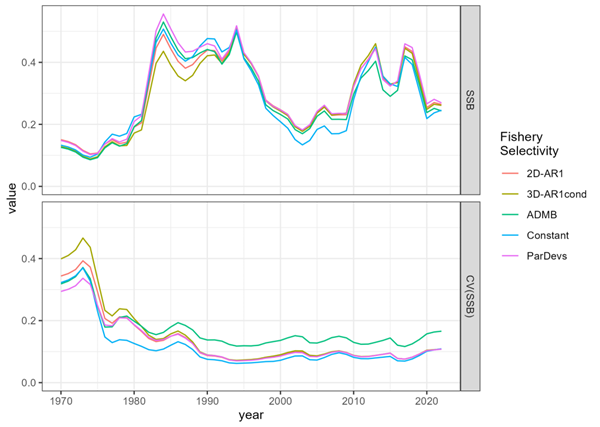
\includegraphics{Results/Figure3_ssb_timeseries.png} The estimated
annual selectivity at age also had the same general patterns, but with
some important differences. All models estimated selectivity at ages 6-8
near 1 (Figs. 4 \& 5). All models also estimated selectivity at age 2 to
be near zero except for a period of about 2000-2010. For age 3, all
models generally agreed and there appear to be meaningful annual
changes, for example in 2008 selectivity was nearly 0.5, but dropped to
around 0.2 by 2015.

Key differences among models are concentrated in ages 4 and 5. As noted
previously, these are the two ages with poor residuals for the ParDev
approach. The largest differences were starting in 2000, with the two
nonparametric models estimated lower age-4 selectivity (Fig. 5). Age 5
selectivity was always estimated over 0.75 but again there are some
differences annually. Overall, all three models estimated distinct
patterns of age 4 and 5 selectivity. This is somewhat surprising given
the similarity of the 2D and 3D AR(1) approaches. Differences in
estimates in projected years are also meaningful, but described
separately below.

\begin{figure}
\hypertarget{fig:figure4}{%
\centering
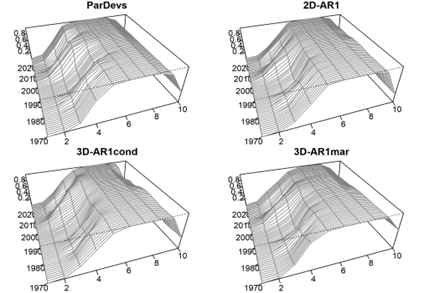
\includegraphics{Results/Figure4_annual_selectivity.png}
\caption{\textbf{Figure 4.} Perspective plots of estimated fisheries
selectivity for candidate models.}\label{fig:figure4}
}
\end{figure}

\begin{figure}
\hypertarget{fig:figure5}{%
\centering
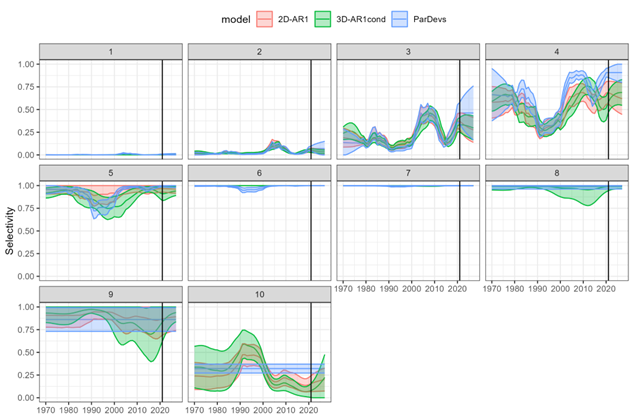
\includegraphics{Results/Figure5_selectivity_at_age_timeseries.png}
\caption{\textbf{Figure 5.} Annual estimates of selectivity at age
(panels) with uncertainty (ribbons, +/- 1 SE) for candidate models. The
last year with fishery age composition is 2021 and denoted with a
vertical line.}\label{fig:figure5}
}
\end{figure}

\hypertarget{model-selection-and-validation}{%
\subsection{Model selection and
validation}\label{model-selection-and-validation}}

OSA residuals for the Constant model show clear patterns and
unexpectedly large OSA residuals (Fig. 6). This justifies more flexible
selectivity forms. The ParDevs model shows much improvement, but still
has lingering patterns in ages 4, 5, and 9, despite having a similar AIC
value. The two non-parametric models eliminated the previous issues, and
have no lingering age or year patterns. There does appear to be a
lingering cohort pattern for the 2012 year class (diagonal positive
residuals).

\begin{figure}
\hypertarget{fig:figure6}{%
\centering
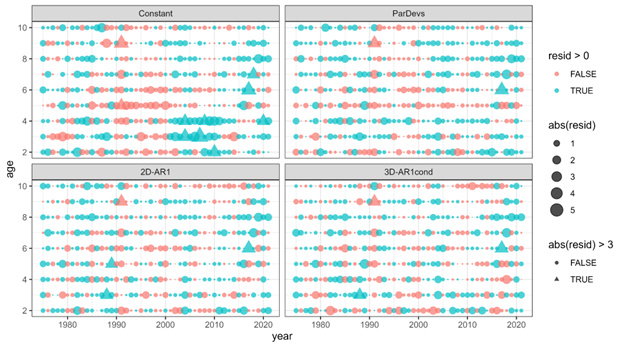
\includegraphics{Results/Figure6_osa_tmb.png}
\caption{\textbf{Figure 6.} OSA residuals for the three candidate models
compared to a model with time-invariant selectivity (Constant).
Residuals are expected to have a standard normal distribution, so
residuals larger than 3 are highlighted as a different
shape.}\label{fig:figure6}
}
\end{figure}

One important property of OSA residuals is that they are expected to
have a standard normal distribution. Standard QQ plots (Fig. 7) show
that the unexpectedly large residuals using the Constant model are
eliminated by the three time-varying selectivity models. However, there
still seem to be some distributional issues remaining, although we judge
this to be of minor concern. We do note that the QQ plots for the two
non-parametric models appear slightly better than the ParDevs approach
currently used in 19.1a.

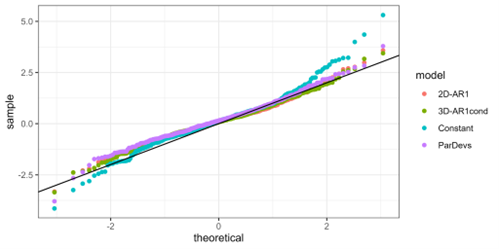
\includegraphics{Results/Figure7_qqplot.png} \#\# Projection performance

Fisheries selectivity for the current assessment year has no fisheries
age composition data and so needs to be extrapolated by the assessment
model. Further, reference point and ABC calculations rely on estimates
of selectivity in the following year. These projected selectivities are
expected to vary among models. The ParDevs model which has a random walk
on parameters will have the same prediction as the last year with data,
but increasing uncertainty with further extrapolation into the future
(Fig. 8). The two AR(1) models will converge toward their stationary
means, but the addition of the cohort effect for the 3D method will
affect the estimates and transitory behavior toward the mean. For many
ages there is little meaningful difference. The age with the most
divergence among models is age 4, where selectivity is 0.91 for the
ParDevs, 0.68 for the 2D-AR1 model, and 0.63 for the 3D-AR1 model.
Interestingly the selectivity is increasing for the 2D model and
decreasing for the 3D model for this age. We hypothesize this is caused
by a cohort effect, although it is not strictly statistically
significant.

\begin{figure}
\hypertarget{fig:figure8}{%
\centering
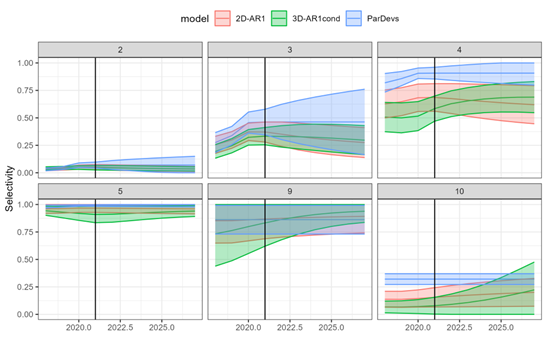
\includegraphics{Results/Figure8_projected_sel.png}
\caption{\textbf{Figure 8.} Behavior of the selectivity modules when
projecting past the last year with fishery age comp data (2021; vertical
line). Annual estimates of selectivity at age (panels) with uncertainty
(ribbons, +/- 1 SE) for candidate models. Ages 1, 6,7 and 8 are left off
for visual clarity as they are nearly constant at 0 or 1 (see Fig. 5).
The ParDev model is a random walk so its projections are constant with
increasing uncertainty. The 2D-AR1 model reverts back to its stationary
mean. The 3D-AR1 model accounts for cohort effects and thus behaves
slightly differently from the 2D version.}\label{fig:figure8}
}
\end{figure}

There are thus important differences, especially in younger ages, for
the predicted selectivity at the two important extrapolated years (Fig.
9).

\begin{figure}
\hypertarget{fig:figure9}{%
\centering
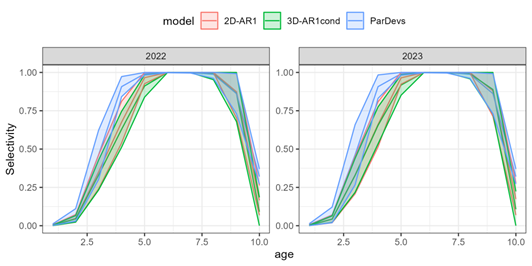
\includegraphics{Results/Figure9_selectivity_at_age_projections.png}
\caption{\textbf{Figure 9.} Estimated selectivity with uncertainty (+/-
1 SE) for the three models in the two important projection
years.}\label{fig:figure9}
}
\end{figure}

\hypertarget{conclusions}{%
\section{Conclusions}\label{conclusions}}

Moving from ADMB to TMB has a few minor disadvantages which are clearly
outweighed by the advantage of being able to estimate hierarchical
models in a statistically defensible way. Hierarchical or ``state
space'' models are now considered ``best practices'' for stock
assessment (Punt 2023) and TMB is the best available tool to accommodate
that framework. We were able to bridge from the ADMB model 19.1a to
within a very small degree of error. \textbf{As such we recommend
retiring the ADMB model and proceeding with model 23 in TMB for use
moving forward. } This modeling framework will allow for important
future extensions beyond fisheries selectivity as well (e.g., maturity
and weight at age smoothing internally).

It is also clear that fisheries selectivity varies over time and that
the current approach of random walk parameter deviations (ParDev model)
is insufficiently flexible for some ages, as determined by residual
patterns. The semi-parametric models explored here did not perform well,
for reasons that are not completely clear at the moment. But two of the
non-parametric models were very promising and had improved residual
patterns. The 3D model had the lowest AIC, with the 2D model about 10
units worse. We believe both non-parametric models would make for
improved fits and projected selectivities for use in calculating
management quantities. The major disadvantage of the non-parametric
models is that they are about 10 times slower to fit than the parametric
version with annual deviates (ParDevs), going from 4 to 40 minutes to
optimize and do the delta method calculations.

Estimating non-parametric components within an assessment takes care, as
putting flexibility in the wrong component can lead to poor management
advice (Szuwalski, Ianelli, and Punt 2018; Fisch et al. 2023). We feel
confident that selectivity does vary through time, and that the forms
examined here do a good job at capturing this change. The new forms also
did not lead to major changes in status, trend, or reference points
among different selectivity options, but there is a remaining
discrepancy when compared to 19.1a that we need to investigate and
resolve. Overall, we conclude that either non-parametric option would
make for an improved model, with the 3D version fitting slightly better
and having a cohort effect, but being more difficult to estimate. We
therefore propose models 23.0a as 23 but with 2D AR(1) fisheries
selectivity, and 23.0b with 3D AR(1) conditional variance. \textbf{We
leave it up to the PT discretion whether to adopt these models this
year.}

\hypertarget{references}{%
\section*{References}\label{references}}
\addcontentsline{toc}{section}{References}

\hypertarget{refs}{}
\begin{CSLReferences}{1}{0}
\leavevmode\vadjust pre{\hypertarget{ref-Cheng2023}{}}%
Cheng, Matthew LH, James T. Thorson, James N. Ianelli, and Curry J.
Cunningham. 2023. {``{Unlocking the triad of age, year, and cohort
effects for stock assessment: Demonstration of a computationally
efficient and reproducible framework using weight-at-age}.''}
\emph{Fisheries Research} 266 (June): 106755.
\url{https://doi.org/10.1016/j.fishres.2023.106755}.

\leavevmode\vadjust pre{\hypertarget{ref-Fisch2023}{}}%
Fisch, N, K Shertzer, E Camp, M Maunder, and R Ahrens. 2023. {``{Process
and sampling variance within fisheries stock assessment models:
estimability, likelihood choice, and the consequences of incorrect
specification}.''} \emph{ICES Journal of Marine Science}, no. September:
2125--49. \url{https://doi.org/10.1093/icesjms/fsad138}.

\leavevmode\vadjust pre{\hypertarget{ref-Kristensen2015}{}}%
Kristensen, Kasper, Anders Nielsen, Casper W Berg, Hans Skaug, and
Bradley M. Bell. 2016. {``{TMB : Automatic Differentiation and Laplace
Approximation}.''} \emph{Journal of Statistical Software} 70 (5): 1--21.
\url{https://doi.org/10.18637/jss.v070.i05}.

\leavevmode\vadjust pre{\hypertarget{ref-Maunder2013}{}}%
Maunder, Mark N., and André E. Punt. 2013. {``{A review of integrated
analysis in fisheries stock assessment}.''} \emph{Fisheries Research}
142: 61--74. \url{https://doi.org/10.1016/j.fishres.2012.07.025}.

\leavevmode\vadjust pre{\hypertarget{ref-Nielsen2014}{}}%
Nielsen, Anders, and Casper W. Berg. 2014. {``{Estimation of
time-varying selectivity in stock assessments using state-space
models}.''} \emph{Fisheries Research} 158: 96--101.
\url{https://doi.org/10.1016/j.fishres.2014.01.014}.

\leavevmode\vadjust pre{\hypertarget{ref-Privitera-Johnson2022}{}}%
Privitera-Johnson, Kristin M., Richard D. Methot, and André E. Punt.
2022. {``{Towards best practice for specifying selectivity in
age-structured integrated stock assessments}.''} \emph{Fisheries
Research} 249 (January).
\url{https://doi.org/10.1016/j.fishres.2022.106247}.

\leavevmode\vadjust pre{\hypertarget{ref-Punt2023}{}}%
Punt, André E. 2023. {``{Those who fail to learn from history are
condemned to repeat it: A perspective on current stock assessment good
practices and the consequences of not following them}.''}
\emph{Fisheries Research} 261 (January).
\url{https://doi.org/10.1016/j.fishres.2023.106642}.

\leavevmode\vadjust pre{\hypertarget{ref-Punt2014}{}}%
Punt, André E., Felipe Hurtado-Ferro, and Athol R. Whitten. 2014.
{``{Model selection for selectivity in fisheries stock assessments}.''}
\emph{Fisheries Research} 158: 124--34.
\url{https://doi.org/10.1016/j.fishres.2013.06.003}.

\leavevmode\vadjust pre{\hypertarget{ref-Skaug2006}{}}%
Skaug, Hans J., and David A. Fournier. 2006. {``{Automatic approximation
of the marginal likelihood in non-Gaussian hierarchical models}.''}
\emph{Computational Statistics and Data Analysis} 51 (2): 699--709.
\url{https://doi.org/10.1016/j.csda.2006.03.005}.

\leavevmode\vadjust pre{\hypertarget{ref-Stock2021}{}}%
Stock, Brian C., and Timothy J. Miller. 2021. {``{The Woods Hole
Assessment Model (WHAM): A general state-space assessment framework that
incorporates time- and age-varying processes via random effects and
links to environmental covariates}.''} \emph{Fisheries Research} 240
(April): 105967. \url{https://doi.org/10.1016/j.fishres.2021.105967}.

\leavevmode\vadjust pre{\hypertarget{ref-Szuwalski2018}{}}%
Szuwalski, Cody S., James N. Ianelli, and André E. Punt. 2018.
{``{Reducing retrospective patterns in stock assessment and impacts on
management performance}.''} \emph{ICES Journal of Marine Science} 75
(2): 596--609. \url{https://doi.org/10.1093/icesjms/fsx159}.

\leavevmode\vadjust pre{\hypertarget{ref-Trijoulet2023}{}}%
Trijoulet, Vanessa, Christoffer Moesgaard Albertsen, Kasper Kristensen,
Christopher M. Legault, Timothy J. Miller, and Anders Nielsen. 2023.
{``{Model validation for compositional data in stock assessment models:
Calculating residuals with correct properties}.''} \emph{Fisheries
Research} 257 (July 2022): 106487.
\url{https://doi.org/10.1016/j.fishres.2022.106487}.

\leavevmode\vadjust pre{\hypertarget{ref-Xu2019}{}}%
Xu, Haikun, James T. Thorson, Richard D. Methot, and Ian G. Taylor.
2019. {``{A new semi-parametric method for autocorrelated age-and
time-varying selectivity in age-structured assessment models}.''}
\emph{Canadian Journal of Fisheries and Aquatic Sciences} 76 (2):
268--85. \url{https://doi.org/10.1139/cjfas-2017-0446}.

\end{CSLReferences}

\end{document}
